\documentclass{article}

% Required packages
\usepackage{amssymb}
\usepackage{amsmath}
\usepackage{graphicx}
\usepackage{geometry}
\usepackage{tikz}
\usepackage{array}
\usepackage{booktabs}
\usepackage{enumitem}
\usepackage{listings}
\usepackage{xcolor}
\usepackage{fancyhdr}
\usepackage{float}
\usepackage{subcaption}
\usepackage{comment}

% Set page geometry
\geometry{a4paper, margin=1in}

% Configure listings for Python
\lstset{
  language=Python,
  basicstyle=\ttfamily\footnotesize,
  numbers=left,
  numberstyle=\tiny\color{gray},
  frame=single,
  breaklines=true,
  breakatwhitespace=true,
  captionpos=b,
  tabsize=4,
  showspaces=false,
  showstringspaces=false,
  showtabs=false,
  commentstyle=\color{gray}\textit,
  keywordstyle=\color{blue}\bfseries,
  stringstyle=\color{red}
}

\begin{document}

\pagestyle{fancy}
\chead{DSC 255: Machine Learning Fundamentals (Spring 2025)}
\lhead{Homework 9}
\rhead{Randall Rogers}

%------------------
% Solution for (a)
%------------------
\subsection*{Solution 1 (a)}
\noindent\rule{\textwidth}{0.4pt}

\subsubsection*{Step 1: Linear Classifiers}
\parbox{\textwidth}{
A single hyperplane can only separate data that is linearly separable. It cannot capture non-linear relationships or create complex, disjoint decision regions.
}

\subsubsection*{\normalfont}{$\therefore$ Linear classifiers are not as expressive as decision trees and cannot represent any arbitrary decision boundary.}
%\parbox{\textwidth}{
% Their expressive power is limited to linear separations.
%}

\noindent\rule{\textwidth}{0.4pt}

\newpage

%------------------
% Solution for (b)
%------------------
\subsection*{Solution 1 (b)}
\noindent\rule{\textwidth}{0.4pt}

\subsubsection*{Step 1: Support Vector Machines with a Quadratic Kernel}
\parbox{\textwidth}{
A quadratic boundary is more flexible than a linear one and can capture more complex relationships. However, it is still restricted to a second-degree polynomial. It cannot represent all possible decision boundaries and especially those with highly irregular shapes.
}

\subsubsection*{\normalfont}{$\therefore$ A SVM with a quadradic kernel is not as expressive as decision trees and cannot represent any arbitrary decision boundary.}

\noindent\rule{\textwidth}{0.4pt}

\newpage

%------------------
% Solution for (c)
%------------------
\subsection*{Solution 1 (c)}
\noindent\rule{\textwidth}{0.4pt}

\subsubsection*{Step 1:Nearest Neighbor Classifiers}

\parbox{\textwidth}{
As the number of training samples grows ($N \to \infty$), a nearest neighbor classifier can approximate any arbitrarily complex decision boundary and can form intricate and highly non-linear shapes.
}

\subsubsection*{\normalfont}{$\therefore$ Nearest neighbor classifiers (with a sufficient number of diverse training samples) are similar in expressive power to decision trees.}


\noindent\rule{\textwidth}{0.4pt}

\newpage

%------------------
% Solution for (d)
%------------------
\subsection*{Solution 1 (d)}
\noindent\rule{\textwidth}{0.4pt}

\subsubsection*{Step 1: Gaussian Generative Models}
\parbox{\textwidth}{
Lets consider the decision boundary for the following Gaussian generative models:
\begin{itemize}
    \item \textbf{Linear Models:} The decision boundary is linear.
    \item \textbf{Quadratic Models:} The decision boundary can be up to a second degree polynomial.
    \item \textbf{Mixture Models:} The decision boundary can be highly non linear.
\end{itemize}
}


\subsubsection*{\normalfont}{$\therefore$ Gaussian Generative Models with a linear or quadradic decision boundary not as expressive as decision trees and cannot represent any arbitrary decision boundary, while Guasian Mixture Models are as expressive.}


\noindent\rule{\textwidth}{0.4pt}

\newpage

%------------------
% Solution
%------------------
\subsection*{Solution 2}
\noindent\rule{\textwidth}{0.4pt}

\subsubsection*{Step 1: Number of Ways to Choose a Feature}
\parbox{\textwidth}{
  Let, $S$ be a set consisting of $n$ data points in a d-dimensional space. 
  If we assume an even distribution of $n$ points across all dimensions $d$ of the set $S$, then the probability of selecting a single point $n_i$(feature) such that it belongs to a single axis of $d$ is $\frac{1}{d}$.
  Hence, we have $d$ potential ways to choose a feature.
}

\subsubsection*{Step 2: Effective Number of Splits for a Chosen Feature}
\parbox{\textwidth}{
If we assume a feature is chosen, and sort the $n$ points. It follows that there exist at most $n-1$ unique midpoints or split points. 
Hence, there are roughly $n-1$ possible splits given one feature has been selected.
}

\subsubsection*{Step 3: Total Number of Possible Splits to Try}
\parbox{\textwidth}{
  From \textbf{Step 1} we know there is $d$ features to choose from and from \textbf{Step 2} we know the maximum number of splits is $n-1$.
  It follows that there exists, $d \times (n-1)$ possibilities to try.
}

\subsubsection*{\normalfont}{$\therefore$ When starting at the top node of a decision tree, we have $d \times (n-1)$ possibilities to try.}

\noindent\rule{\textwidth}{0.4pt}

\newpage

%------------------
% Solution
%------------------
\subsection*{Solution 3}
\noindent\rule{\textwidth}{0.4pt}

\subsubsection*{Step 1}
\parbox{\textwidth}{
  The Gini impurity index ($GII$) is defined as the following where $p$ is the probability of one label and $1-p$ is the probability of the second label:
  $$GII=2p(1-p)$$
  By the commutative property of multiplication it doe not matter what value we choose for $p$ since the result will be the same.
}

\subsubsection*{Step 2: Calculate the Gini Impurity Index}
\parbox{\textwidth}{
Let $p=0.2$ and subsitute into the Gini impurity formula:
$$GII=2p(1-p)$$
$$GII=2\cdot(0.2)\cdot(1-0.2)$$
$$GII=0.32$$
}

\subsubsection*{\normalfont}{$\therefore$ The Gini impurity index for a node in which 20\% of the points have one label and 80\% have the other label is 0.32.}

\noindent\rule{\textwidth}{0.4pt}

\newpage

%------------------
% Solution for (a) - Decision Trees
%------------------
\subsection*{Solution 4 (a)}
\noindent\rule{\textwidth}{0.4pt}

\subsubsection*{Step 1}
\parbox{\textwidth}{
To incorporate weights $\lambda_i$ into decision trees, we modify how we calculate the proportion of points belonging to each class at a given node. 
It follows that, incorprating weighted data would only impact the impurity calculation.\\

Let $S$ be a set that contains all data points at a particular node. The weighted proportion $p_k$ for class $k$ at this node is calculated as the sum of weights of points in class $k$ divided by the total sum of weights of all points at the node:
$$ p_k = \frac{\sum_{i \in S_k} \lambda_i}{\sum_{j \in S} \lambda_j} $$

}
\subsubsection*{\normalfont}{$\therefore$These weighted proportions $\sum_{k} p_k = 1$ are then used in the impurity measures.}

\noindent\rule{\textwidth}{0.4pt}

\newpage

%------------------
% Solution for (b) - Gaussian Generative Models
%------------------
\subsection*{Solution 4 (b)}
\noindent\rule{\textwidth}{0.4pt}

\subsubsection*{Step 1}
\parbox{\textwidth}{
To incorporate weights $\lambda_i$ into a Gaussian generative model, we must adjust the calculations of the class prior, weighted mean, and covariance.
}

\subsubsection*{Step 2: Weighted Class Priors ($\pi_j$)}
\parbox{\textwidth}{
In a Gaussian generative model, the class prior $\pi_j = P(C_j)$ is the fraction of training samples belonging to class $j$. With weighted data, let $N$ be the total number of data points. Let $I_j$ be the set of indices of data points belonging to class $j$. The weighted class prior $\pi_j$ is the sum of weights of samples in class $j$ divided by the total sum of weights of all samples:
$$ \pi_j = \frac{\sum_{i \in I_j} \lambda_i}{\sum_{m=1}^{N} \lambda_m} $$
}

\subsubsection*{Step 3: Weighted Mean ($\boldsymbol{\mu}_j$)}
\parbox{\textwidth}{
The mean $\boldsymbol{\mu}_j$ for class $j$ is the average of the feature vectors $\mathbf{x}^{(i)}$ belonging to class $j$. For weighted data, this becomes a weighted average:
$$ \boldsymbol{\mu}_j = \frac{\sum_{i \in I_j} \lambda_i \mathbf{x}^{(i)}}{\sum_{i \in I_j} \lambda_i} $$
Each data point $\mathbf{x}^{(i)}$ in class $j$ contributes to the mean proportionally to its weight $\lambda_i$.
}

\subsubsection*{Step 4: Weighted Covariance Matrix ($\boldsymbol{\Sigma}_j$)}
\parbox{\textwidth}{
The covariance matrix $\boldsymbol{\Sigma}_j$ for class $j$ measures the spread and correlation of features for that class. For weighted data, it is estimated as:
$$ \boldsymbol{\Sigma}_j = \frac{\sum_{i \in I_j} \lambda_i (\mathbf{x}^{(i)} - \boldsymbol{\mu}_j)(\mathbf{x}^{(i)} - \boldsymbol{\mu}_j)^T}{\sum_{i \in I_j} \lambda_i} $$
}

\subsubsection*{\normalfont}{$\therefore$ For Gaussian generative models, sample weights $\lambda_i$ are incorporated by using weighted sums to estimate the class priors $\pi_j$, class means $\boldsymbol{\mu}_j$, and class covariance matrices $\boldsymbol{\Sigma}_j$}

\noindent\rule{\textwidth}{0.4pt}

\newpage

%------------------
% Solution for (c) - Support Vector Machines
%------------------
\subsection*{Solution 4 (c)}
\noindent\rule{\textwidth}{0.4pt}

\subsubsection*{Step 1}
\parbox{\textwidth}{
The objective function for a soft-margin linear SVM is defined as:
$$ \min_{\mathbf{w}, b, \boldsymbol{\xi}} \frac{1}{2} \|\mathbf{w}\|^2 + C \sum_{i=1}^{N} \xi_i $$
such that:
$$ y^{(i)}(\mathbf{w}^T \mathbf{x}^{(i)} + b) \ge 1 - \xi_i, \quad \xi_i \ge 0 \quad \text{for } i=1, \ldots, N $$
Where $C$ is the regularization parameter that balances margin maximization and misclassification penalty, and $\xi_i$ are slack variables allowing for misclassifications.
}

\subsubsection*{Step 2}
\parbox{\textwidth}{
To incorporate sample weights into the objective function for a soft-margin linear SVM, we must modify the penalty term for the slack variables. Points with higher weights will incur a larger penalty if they are misclassified or fall within the margin. The objective function becomes:
$$ \min_{\mathbf{w}, b, \boldsymbol{\xi}} \frac{1}{2} \|\mathbf{w}\|^2 + C \sum_{i=1}^{N} \lambda_i \xi_i $$
such that:
$$ y^{(i)}(\mathbf{w}^T \mathbf{x}^{(i)} + b) \ge 1 - \xi_i, \quad \xi_i \ge 0 \quad \text{for } i=1, \ldots, N $$
}

\subsubsection*{\normalfont}{$\therefore$ For Support Vector Machines, sample weights $\lambda_i$ are incorporated by modifying the objective function to penalize errors on high-weight samples more heavily.}

\noindent\rule{\textwidth}{0.4pt}

\newpage

%------------------
% Solution for (a)
%------------------
\subsection*{Solution 5 (a)}
\noindent\rule{\textwidth}{0.4pt}

\subsubsection*{Step 1}
\parbox{\textwidth}{
  Boosting algorithms, are designed to minimize an objective function related to the training error. The condition that the weak learner's error is at most $\tfrac12 - \epsilon$ ensures that boosting can effectively reduce training error, but it doesn't control for the inherent generalization gap between training and test performance.
}

\subsubsection*{\normalfont}{$\therefore$ The statement "Boosting converges to a final classifier with zero test error" is \textbf{False}.}


\noindent\rule{\textwidth}{0.4pt}

\newpage

%------------------
% Solution for (b)
%------------------
\subsection*{Solution 5 (b)}
\noindent\rule{\textwidth}{0.4pt}

\subsubsection*{Step 1}
\parbox{\textwidth}{
  The condition that each weak learner $h_t$ has a weighted error $\text{err}_t \le \frac{1}{2} - \epsilon$ (where $\epsilon > 0$) ensures that each weak learner performs better than random guessing on the current distribution of weights.
  It follows that the training error would converge to zero over enough itterations.
}

\subsubsection*{\normalfont}{$\therefore$ The statement "Boosting converges to a final classifier with zero training error" is \textbf{True} (under the given conditions and assuming enough iterations).}


\noindent\rule{\textwidth}{0.4pt}

\newpage

%------------------
% Solution for (c)
%------------------
\subsection*{Solution 5 (c)}
\noindent\rule{\textwidth}{0.4pt}

\subsubsection*{Step 1}
\parbox{\textwidth}{
The class $\mathcal H$ represents the set of possible \emph{weak} classifiers and the final classifier produced by boosting, $H(\mathbf{x})$, is a weighted linear combination of these weak classifiers.
While each weak learner is an element of $\mathcal H$, the subsquent sum of weak learners and boosting can form a complex non-linear decision boundary. Hence, the final classifier would not nessicarily be an element of $\mathcal H$.
}

\subsubsection*{\normalfont}{$\therefore$ The statement "Boosting's final classifier belongs to class $\mathcal H$" is \textbf{False}.}

\noindent\rule{\textwidth}{0.4pt}

\newpage

%------------------
% Solution for (a)
%------------------
\subsection*{Solution 6 (a)}
\noindent\rule{\textwidth}{0.4pt}

\subsubsection*{Step 1}
\parbox{\textwidth}{
In a Random Forest, each decision tree is trained independently of the others. Each tree is built using a different bootstrap sample of the training data and considers a random subset of features at each split. Since the construction of one tree does not depend on the outcome or structure of any other tree, their training processes can be executed in parallel.
}

\subsubsection*{\normalfont}{$\therefore$ The statement: \textit{The trees can be trained in parallel.} is \textbf{True} }

\noindent\rule{\textwidth}{0.4pt}

\newpage

%------------------
% Solution for (b)
%------------------
\subsection*{Solution 6 (b)}
\noindent\rule{\textwidth}{0.4pt}

\subsubsection*{Step 1}
\parbox{\textwidth}{
Individual trees in a Random Forest are typically grown to a large depth. They are trained to fit their respective bootstrap samples of the data as well as possible. Hence, each tree is \textit{optimized} to capture the patterns in the subset of data it sees, and is a reason why random forests have an issue of overfitting the training data.
}

\subsubsection*{\normalfont}{$\therefore$ The statement: \textit{Each individual tree is more highly optimized.} is \textbf{True}.}

\noindent\rule{\textwidth}{0.4pt}

\newpage

%------------------
% Solution for (c)
%------------------
\subsection*{Solution 6 (c)}
\noindent\rule{\textwidth}{0.4pt}

\subsubsection*{Step 1}
\parbox{\textwidth}{
From \textbf{Solution 6 (b)}, we know that individual trees in a Random Forest are grown to a large depth and each individual tree is trained trained to fit their respective bootstrap samples of the data as well as possible. 
Conversely, bossted decision trees on require slightly better accuracy on the training data than random guessing.
}

\subsubsection*{\normalfont}{$\therefore$ The statement: \textit{Each individual tree has better accuracy.} is \textbf{True}.}

\noindent\rule{\textwidth}{0.4pt}

\newpage


\subsection*{Solution 7 (a)}
\noindent\rule{\textwidth}{0.4pt}\\

\subsubsection*{Sneak Preview at mini-data.txt}

\begin{figure}[H]
  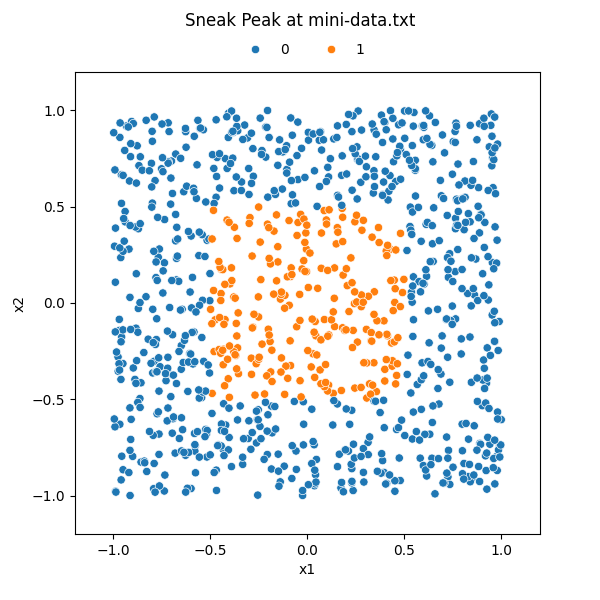
\includegraphics{hw9_q7a.png}
  \caption{Sneak Peak of mini-data.txt, reveals a square doughnut shape.}
\end{figure}

\noindent\rule{\textwidth}{0.4pt}\\

\newpage

\subsection*{Solution 7 (b)}
\noindent\rule{\textwidth}{0.4pt}\\

\subsubsection*{DecisionTreeClassifier: Stop condition}
\begin{table}[h!]               
  \centering                    
  \begin{tabular}{|c|c|c|}
    \hline
    Max depth & Training accuracy & Test accuracy \\ \hline
    1 & 0.50 & 0.49 \\ 
    2 & 0.76 & 0.75 \\ 
    3 & 0.88 & 0.90 \\ 
    4 & 1.00 & 1.00 \\ \hline
  \end{tabular}
  \caption{The stop condition selected was \texttt{max\_depth=4}}   
  \label{tab:depth_accuracy}
\end{table}

\subsubsection*{Python Code}
\begin{lstlisting}
from sklearn.tree import DecisionTreeClassifier
from sklearn.model_selection import train_test_split

x_train, x_test, y_train, y_test = train_test_split(x_data,
                                                    y_data,
                                                    test_size=0.2,
                                                    random_state=42)

def dtc_q7(x_train, x_test, y_train, y_test,n):
    dtc = DecisionTreeClassifier(criterion='log_loss',
                                 max_depth=n,
                                 max_leaf_nodes=n+1,
                                 class_weight='balanced',
                                 min_samples_leaf=int(len(x_train)*0.015),
                                 random_state=42)
    dtc.fit(x_train,y_train)
    print(f"train score(max_depth={n}): {dtc.score(x_train,y_train)}")
    print(f"test score(max_depth={n}): {dtc.score(x_test,y_test)}")

for n in range(1,5):
    dtc_q7(x_train, x_test, y_train, y_test,n)
\end{lstlisting}


\noindent\rule{\textwidth}{0.4pt}\\

\newpage

\subsection*{Solution 7 (c)}
\noindent\rule{\textwidth}{0.4pt}\\

\subsubsection*{Plot}
\begin{figure}[H]
  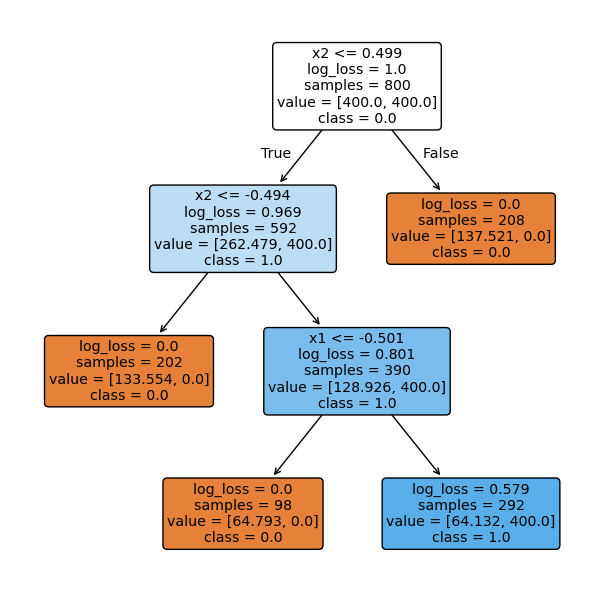
\includegraphics{hw9_q7c.png}
  \caption{Tree plot from the decision tree classifier.}
\end{figure}

\noindent\rule{\textwidth}{0.4pt}\\

\newpage

\subsection*{Solution 7 (d)}
\noindent\rule{\textwidth}{0.4pt}\\
\subsubsection*{Stump Plots}
\begin{center}
  \begin{figure}[H]
    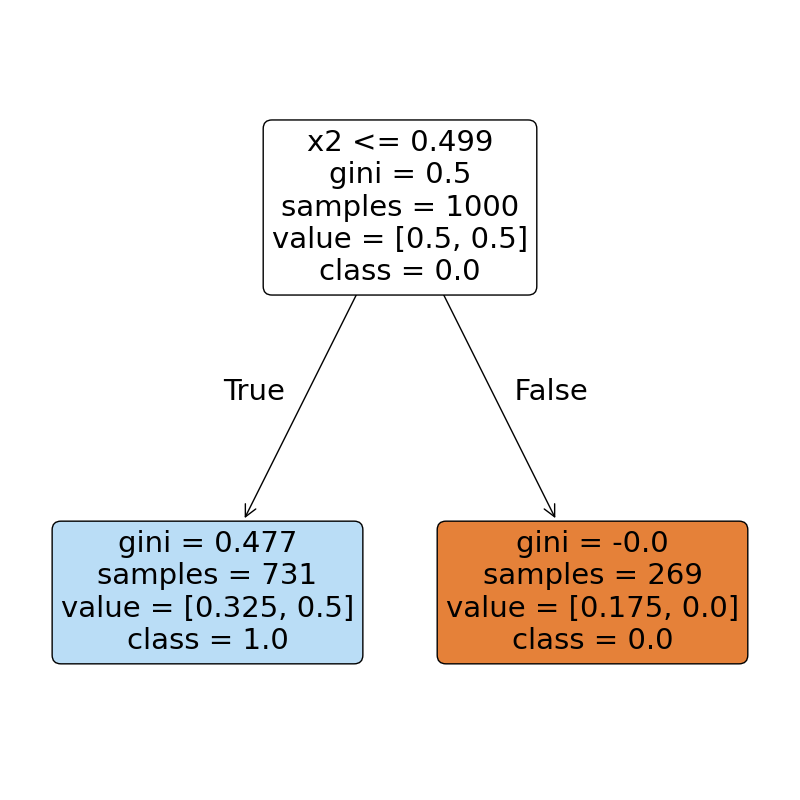
\includegraphics{hw9_q7d_ada_stumps_1.png}
    \caption{Tree plot from the ada boost with one stump}
  \end{figure}
\end{center}

\begin{center}
  \begin{figure}[H]
    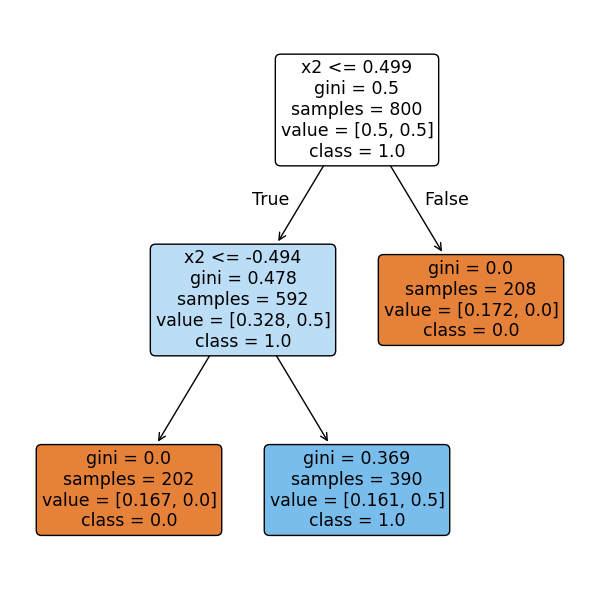
\includegraphics{hw9_q7d_ada_stumps_2.png}
    \caption{Tree plot from the ada boost with two stumps}
  \end{figure}
\end{center}

\begin{center}
  \begin{figure}[H]
    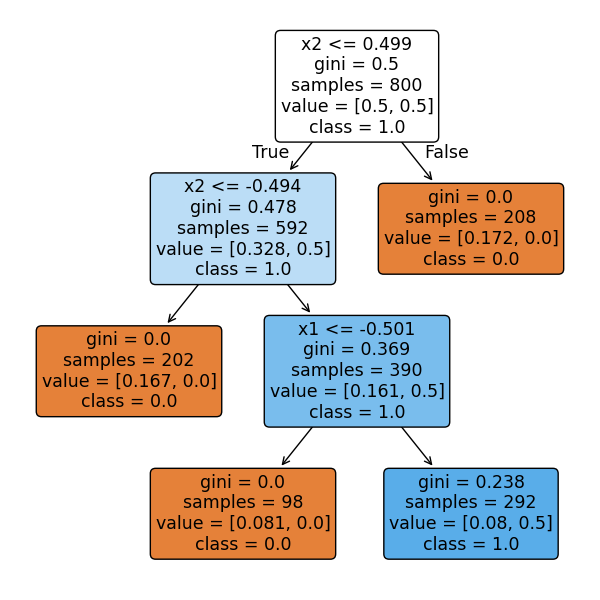
\includegraphics{hw9_q7d_ada_stumps_3.png}
    \caption{Tree plot from the ada boost with three stumps}
  \end{figure}
\end{center}


\noindent\rule{\textwidth}{0.4pt}\\

\newpage

\subsection*{Solution 7 (e)}
\noindent\rule{\textwidth}{0.4pt}\\

\subsubsection*{Ada Boost Training Accuracy}
\begin{table}[h!]               
  \centering                    
  \begin{tabular}{|c|c|}
    \hline
    Stumps & Training accuracy \\ \hline
    1 & 0.50 \\ 
    2 & 0.73 \\ 
    3 & 1.00 \\ \hline
  \end{tabular}
  \caption{The training accuracy of the ada boost model increased as the number of stumps increased.}   
  \label{tab:trainacc}
\end{table}

\subsubsection*{Python Code}
\begin{lstlisting}
  from sklearn.ensemble import AdaBoostClassifier

  def ada_q7(x_train, x_test, y_train, y_test,n):
      ## initalize the first decision tree stump for the ada booster
      stump = DecisionTreeClassifier(max_depth=n,
                                     class_weight='balanced',
                                     random_state=42)
  
      ## initalize ada booster model with n stumps
      ada = AdaBoostClassifier(estimator=stump,
                               n_estimators=n,
                               learning_rate=1.0,
                               algorithm='SAMME',
                               random_state=42)
  
      ada.fit(x_train,y_train)
      print(f"train score(n_estimators={n}): {ada.score(x_train,y_train)}")
      print(f"test score(n_estimators={n}): {ada.score(x_test,y_test)}")
  
      fig = plt.figure(figsize=(6,6))
      tree.plot_tree(ada.estimators_[0], feature_names=["x1", "x2"], class_names=["0.0","1.0"],filled=True, rounded=True)
      plt.tight_layout()
      plt.savefig(f"hw9_q7d_ada_stumps_{n}.png")
  
  stumps = [1,2,3]
  for n in stumps:
      ada_q7(x_train, x_test, y_train, y_test,n)  
\end{lstlisting}

\noindent\rule{\textwidth}{0.4pt}\\

\newpage

\subsection*{Solution 8 (a)}
\noindent\rule{\textwidth}{0.4pt}\\
\parbox{\textwidth}{Running the following commands tells us the distribution of fradulent and legitimate in \textit{creditcard.csv}}
\begin{itemize}
  \item legitimate (class:0): 284315
  \begin{itemize}
    \item \texttt{cat creditcard.csv | rev | cut -d ',' -f 1 | rev | grep 0 | wc -l}
  \end{itemize}
  \item fradulent (class:1): 492
  \begin{itemize}
    \item \texttt{cat creditcard.csv | rev | cut -d ',' -f 1 | rev | grep 1 | wc -l}
  \end{itemize}
\end{itemize}

\noindent\rule{\textwidth}{0.4pt}\\

\newpage

\subsection*{Solution 8 (b)}
\noindent\rule{\textwidth}{0.4pt}\\

\subsubsection*{Python Code: Downsample}
\begin{lstlisting}
import pandas as pd
from sklearn.model_selection import train_test_split

## read creditcard.csv
cc = pd.read_csv('creditcard.csv')

## split data by class, balance to 50/50, and combine into one dataframe
fraud = cc[cc['Class']==1.0]
legit = cc[cc['Class']==0.0].sample(n=len(fraud),random_state=42)
cc_bal = pd.concat([fraud,legit]).sample(frac=1, random_state=42)

## split balanced dataframe to x,y , convert to numpy arrays and then training and test data sets
x = cc_bal.drop(columns=['Class'],inplace=False).to_numpy()
y = cc_bal['Class'].astype(int).to_numpy()

## split data for models
x_train, x_test, y_train, y_test = train_test_split(x,y,test_size=0.2, random_state=42)
\end{lstlisting}

\noindent\rule{\textwidth}{0.4pt}\\

\newpage

\subsection*{Solution 8 (c)}
\noindent\rule{\textwidth}{0.4pt}\\

\subsubsection*{Python Code: Fit Models}
\begin{lstlisting}
from sklearn.tree import DecisionTreeClassifier
from sklearn.ensemble import AdaBoostClassifier, RandomForestClassifier
from sklearn.model_selection import cross_val_predict, StratifiedKFold
from sklearn.metrics import confusion_matrix, ConfusionMatrixDisplay

def fit_dt(x_train, x_test, y_train, y_test ):
    dt = DecisionTreeClassifier(criterion='gini', max_depth=4, class_weight='balanced', min_samples_leaf=20, random_state=42)
    dt.fit(x_train,y_train)
    cv = StratifiedKFold(n_splits=5, shuffle=True, random_state=42)
    y_pred = cross_val_predict(dt, x_test, y_test, cv=cv)
    cm = confusion_matrix(y_test,y_pred,labels=[0,1])
    cmd = ConfusionMatrixDisplay(confusion_matrix=cm, display_labels=["legit","fraud"])
    cmd.plot(cmap="Blues")
    score = dt.score(x_test,y_test)
    print(f"accuracy of decision tree:(train): {dt.score(x_train,y_train):.3f}")
    print(f"accuracy of decision tree:(test): {score:.3f}")
    cmd.ax_.set_title(f"Decision Tree Classifier\n Test Accuracy: {score:.3f}")
    plt.savefig("dt_classifier.png")

def fit_ada(x_train, x_test, y_train, y_test):
    ada = AdaBoostClassifier(n_estimators=6, algorithm='SAMME',random_state=42)
    ada.fit(x_train,y_train)
    cv = StratifiedKFold(n_splits=5, shuffle=True, random_state=42)
    y_pred = cross_val_predict(ada,x_test,y_test,cv=cv)
    cm = confusion_matrix(y_test,y_pred,labels=[0,1])
    cmd = ConfusionMatrixDisplay(confusion_matrix=cm, display_labels=["legit","fraud"])
    cmd.plot(cmap="Greens")
    score = ada.score(x_test,y_test)
    print(f"accuracy of ada boost(train): {ada.score(x_train,y_train):.3f}")
    print(f"accuracy of ada boost(test): {score:.3f}")
    cmd.ax_.set_title(f"Ada Boost Classifier\n Test Accuracy: {score:.3f}")
    plt.savefig("boost_classifier.png")


def fit_rf(x_train, x_test, y_train, y_test):
    rf = RandomForestClassifier(n_estimators=100, criterion='gini',class_weight='balanced',random_state=42)
    rf.fit(x_train,y_train)
    cv = StratifiedKFold(n_splits=5,shuffle=True,random_state=42)
    y_pred =cross_val_predict(rf,x_test,y_test,cv=cv)
    cm = confusion_matrix(y_test,y_pred,labels=[0,1])
    cmd = ConfusionMatrixDisplay(confusion_matrix=cm, display_labels=["legit","fraud"])
    cmd.plot(cmap="Reds")
    score = rf.score(x_test,y_test)
    print(f"accuracy of random forest(train): {rf.score(x_train,y_train):.3f}")
    print(f"accuracy of random forest(test): {score:.3f}")
    cmd.ax_.set_title(f"Random Forest Classifier\n Test Accuracy: {score:.3f}")
    plt.savefig("rf_classifier.png")


fit_dt(x_train, x_test, y_train, y_test)
fit_ada(x_train, x_test, y_train, y_test)
fit_rf(x_train, x_test, y_train, y_test)

\end{lstlisting}

\newpage

\subsubsection*{Plots: Slick Confusion Matrices}

\begin{center}
  \begin{figure}[H]
    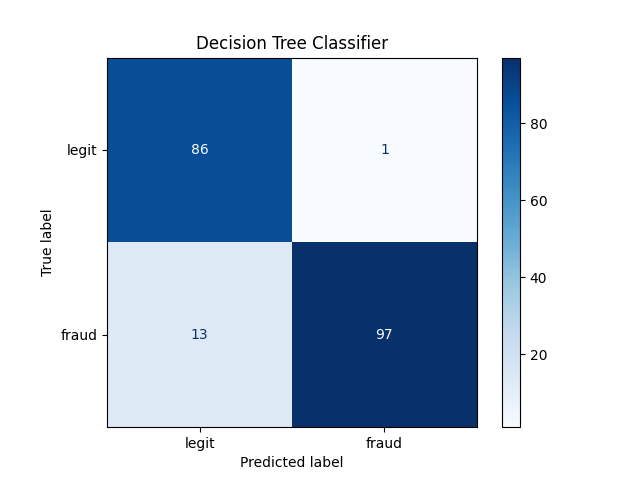
\includegraphics{dt_classifier.png}
    \caption{Confusion matrix for decision tree classifier.}
  \end{figure}
\end{center}

\begin{center}
  \begin{figure}[H]
    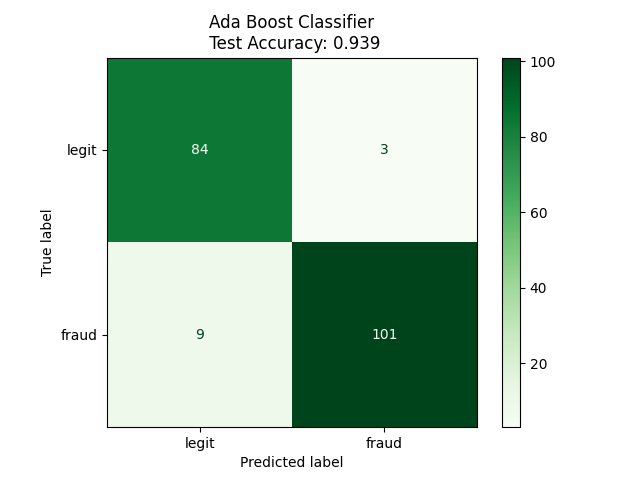
\includegraphics{boost_classifier.png}
    \caption{Confusion matrix for ada boost classifier.}
  \end{figure}
\end{center}

\begin{center}
  \begin{figure}[H]
    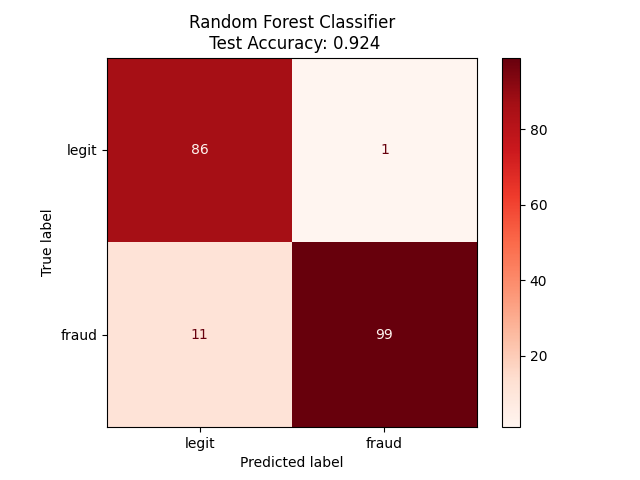
\includegraphics{rf_classifier.png}
    \caption{Confusion matrix for random forest classifier.}
  \end{figure}
\end{center}

\noindent\rule{\textwidth}{0.4pt}\\

\begin{comment}
  \begin{center} 
  \begin{tabular}{|c|c|c|} 
    \hline Stump Number (\%) & Training Accuracy (\%) \\ 
    \hline 
    1 & 16.32\\ 
    2 & 15.91 \\
    3 & 14.25 \\
    4 & 13.56 \\ 
    5 & 14.05  \\ 
    \hline
  \end{tabular}
\end{center}
\end{comment}

\begin{comment}
\subsection*{Solution 7}
\noindent\rule{\textwidth}{0.4pt}\\

\begin{figure}
  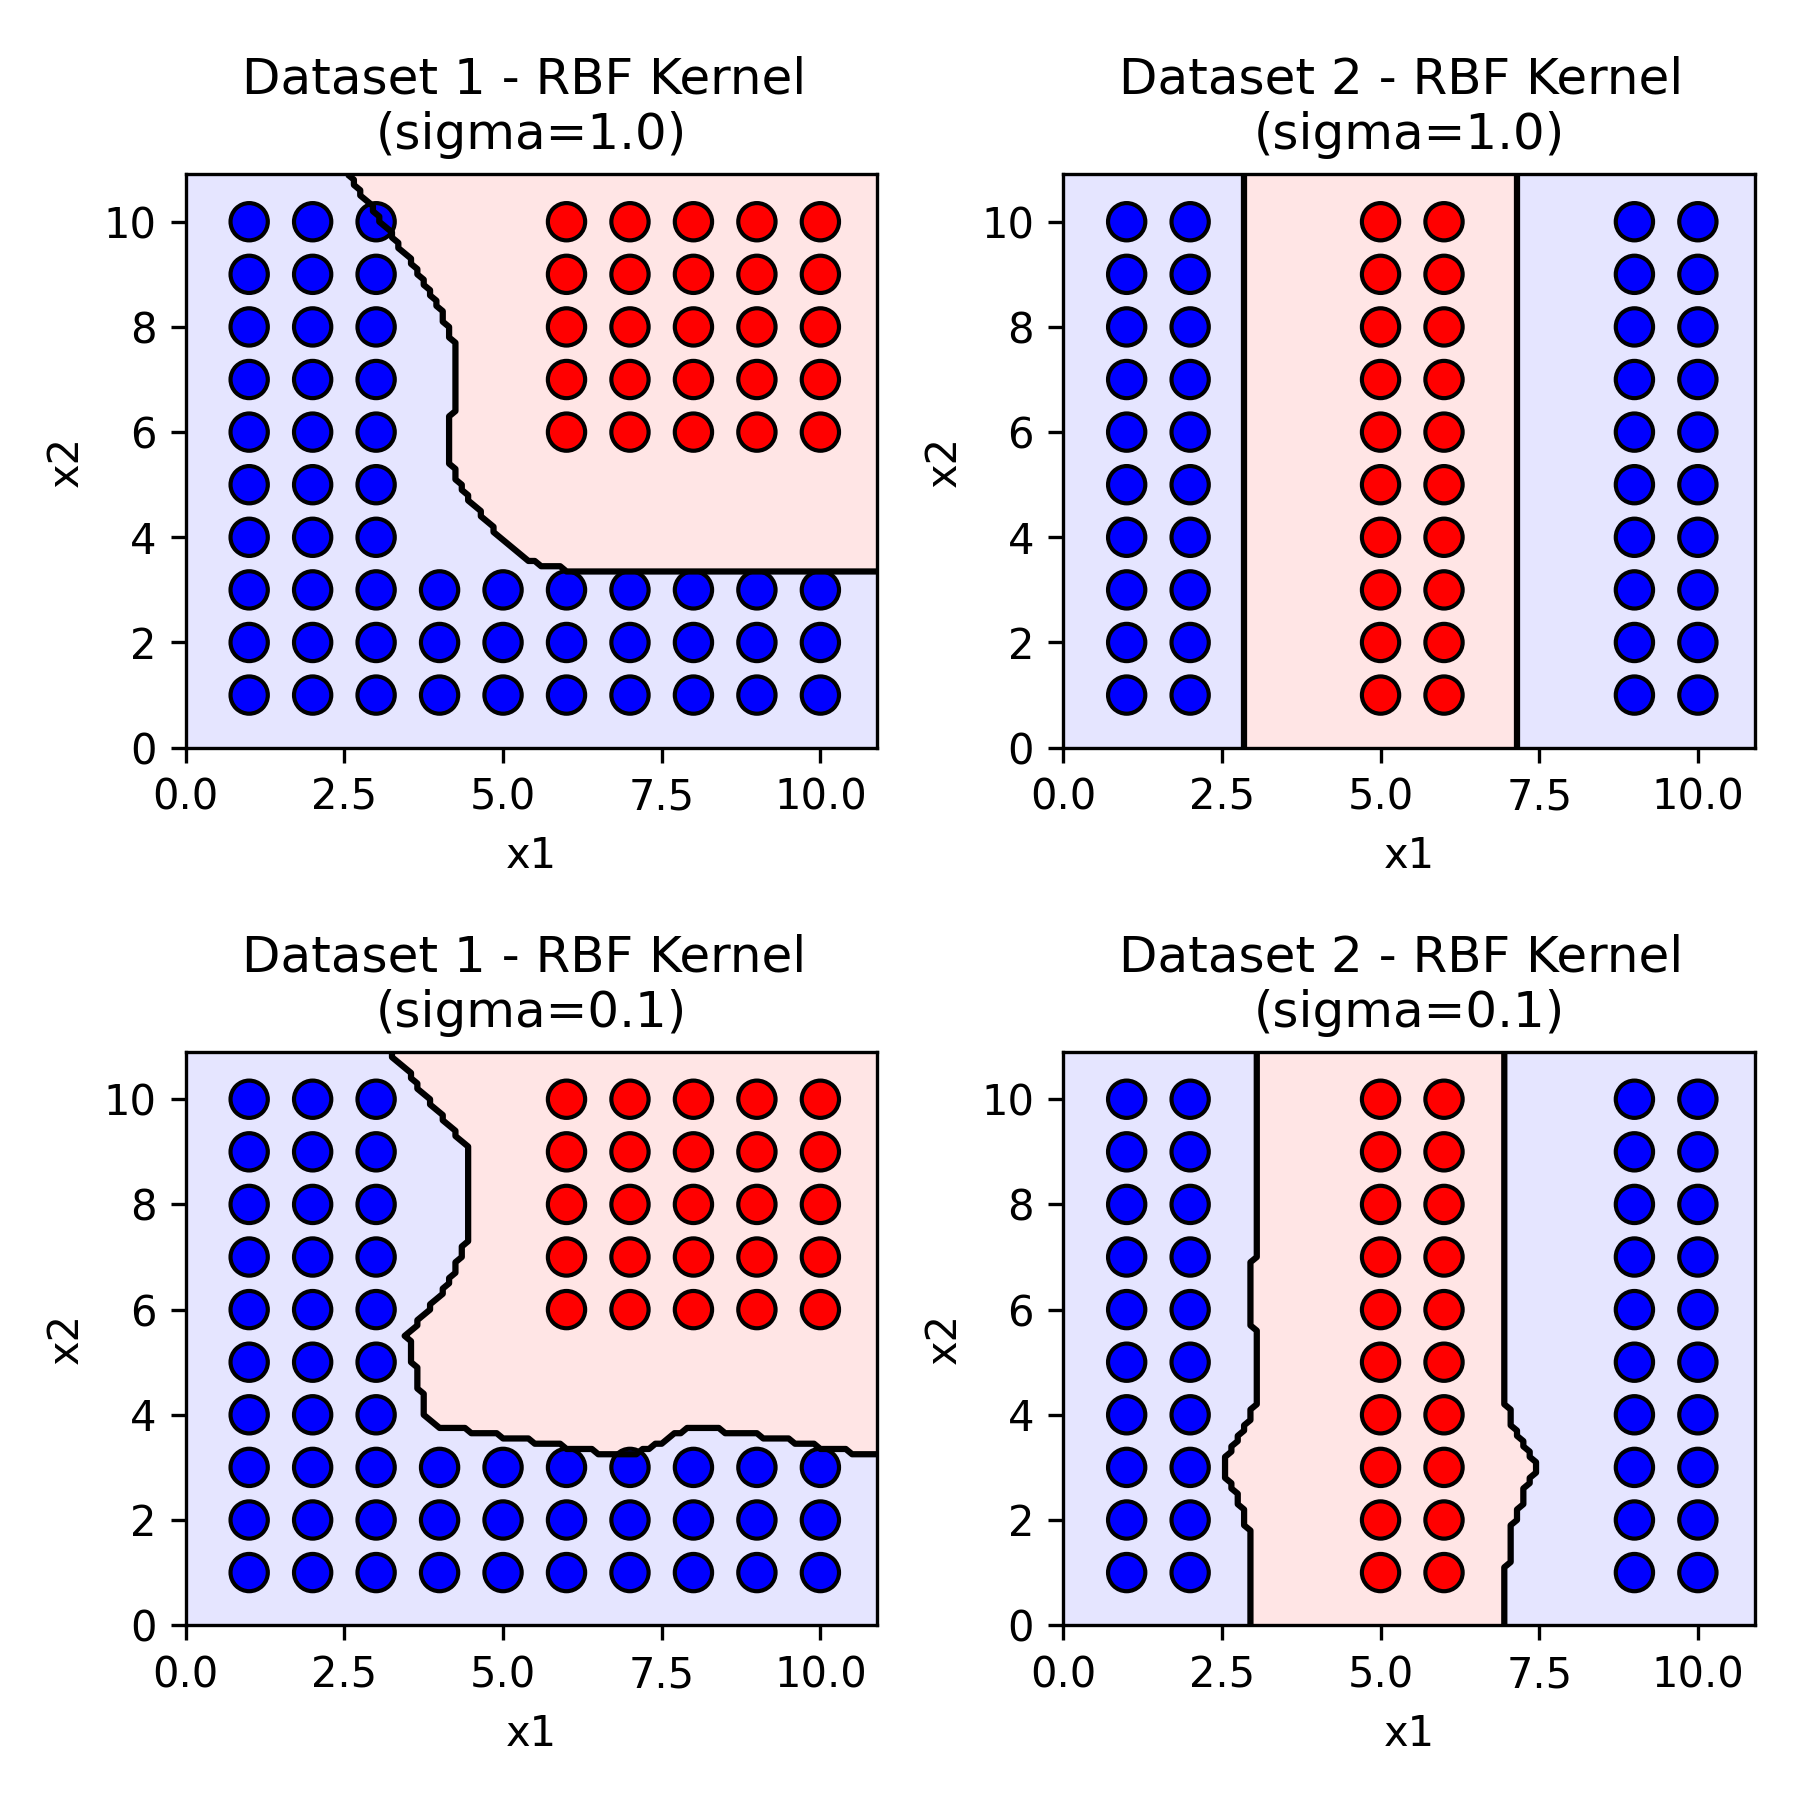
\includegraphics{part_b_rbf_kernel.png}
  \caption{Decision boundary for rbf kernel}
\end{figure}
\noindent\rule{\textwidth}{0.4pt}\\

\subsubsection*{Linear SVM}

\begin{center} 
  \begin{tabular}{|c|c|c|} 
    \hline C Value & Training Error (\%) & Test Error (\%) \\ 
    \hline 
    0.01 & 16.32 & 15.48\\ 
    0.1 & 15.91 & 16.36 \\
    1.0 & 14.25 & 14.04 \\
    10.0 & 13.56 & 13.16 \\ 
    100.0 & 14.05 & 14.78 \\ 
    \hline
  \end{tabular}
\end{center}
\parbox{\textwidth}{Based on the results above it seems that the data is linearly separable.}
\subsubsection*{Quadardic SVM}
\begin{center} 
  \begin{tabular}{|c|c|c|} 
    \hline Training Error (\%) & Test Error (\%)  & Support Vectors\\ 
    \hline 
    0.17 & 2.13 & 17906\\ 
    \hline
  \end{tabular}
\end{center}

\begin{lstlisting}
PYTHON CODE HERE
\end{lstlisting}
\end{comment}
\end{document}

